%\documentclass[journal]{IEEEtran}
%\documentclass[12pt,onecolumn]{IEEEtran}
\documentclass[UTF8]{article}
\usepackage{ctex}
\usepackage{geometry,graphicx,marvosym}
\usepackage{amsmath,amsthm}
\usepackage{amsfonts}
\usepackage[usenames,dvipsnames]{pstricks}
\usepackage{pst-plot,pstricks-add}
%\usepackage{graphicx,times,amsmath,amssymb,multirow,subfigure}
\usepackage{graphicx,times,amsmath,amssymb,multirow}
\usepackage{url}
\usepackage{stfloats}
\usepackage{amsfonts,rotating}
\usepackage{color}
\usepackage{verbatim,multirow}
% setting dimension of the paper
\textwidth 7.0true in
\textheight 8.9 true in
\topmargin=-20pt
\headheight=6pt
\headsep=2pt
\oddsidemargin -0.3true in
\evensidemargin -0.4true in
\usepackage{amssymb}

\newtheorem{theorem}{Theorem}
\newtheorem{lemma}{Lemma}
\newtheorem{algorithm}{Algorithm}
\newtheorem{definition}{Definition}
\newtheorem{proposition}{Proposition}

\newcommand{\dtcwt}{\operatorname{DT-\mathbb{C}WT}}
\newcommand{\tpctf}{\operatorname{TP-\mathbb{C}TF}}
\newcommand{\ctf}{\operatorname{\mathbb{C}TF}}
\newcommand{\tr}[1]{\textcolor{red}{#1}}
\newcommand{\tb}[1]{\textcolor{blue}{#1}}
\newcommand{\mO}{{\mathcal{T}}}
\newcommand{\C}{\mathbb{C}}    %complex number field
\newcommand{\N}{\mathbb{N}}    %natural numbers
\newcommand{\R}{\mathbb{R}}    %real number field
\newcommand{\Z}{\mathbb{Z}}    %integers
\newcommand{\imag}{\mathrm{i}} % imaginary unit
\newcommand{\dR}{\mathbb{R}^d}
\newcommand{\dT}{\mathbb{T}^d}
\newcommand{\dZ}{\mathbb{Z}^d}
\newcommand{\dlp}[1]{l_{#1}(\mathbb{Z}^d)}
\newcommand{\td}{\boldsymbol{\delta}}  %Dirac/Kronicker sequence
\newcommand{\bp}{\begin{proof}}
	\newcommand{\ep}{\hfill  \end{proof} }
\newcommand{\be}{ \begin{equation} }
	\newcommand{\ee}{ \end{equation} }
\newcommand{\dLp}[1]{L_{#1}(\mathbb{R}^d)}
\newcommand{\prm}{P}           %projection matrix
\newcommand{\wh}{\widehat}
\renewcommand{\le}{\leqslant}
\renewcommand{\ge}{\geqslant}
\newcommand{\bs}{\backslash}
\newcommand{\ol}{\overline}
\newcommand{\vk}{\mathsf{k}}
\newcommand{\la}{\langle}
\newcommand{\ra}{\rangle}
\newcommand{\tp}{\mathsf{T}}  %transpose
\newcommand{\conj}{\overline}
\newcommand{\supp}{\mathrm{supp}}
\newcommand{\setsp}{\;:\;}     %set separator
\newcommand{\sd}{\mathcal{S}}  %subdivision operator S
\newcommand{\tz}{\mathcal{T}}  %transition operator T
\newcommand{\wt}{\widetilde}
\renewcommand{\le}{\leqslant}
\renewcommand{\ge}{\geqslant}
\newcommand{\er}{\eqref}
\newcommand{\gep}{\varepsilon}
\newcommand{\eps}{\epsilon}
\newcommand{\gl}{\lambda}
\newcommand{\gL}{\Lambda}
\newcommand{\gd}{\delta}
\newcommand{\DAS}{\mathrm{DAS}}
\newcommand{\UDAS}{\mathrm{UDAS}}
\newcommand{\DHF}{\mathrm{DHF}}
\newcommand{\bm}{\boldmath}
\newtheorem{example}{Example}
\bibliographystyle{unsrt}
\newcommand{\xz}[1]{\textcolor{magenta}{\bf #1}}
\usepackage[colorlinks,linkcolor=blue,anchorcolor=blue,citecolor=blue]{hyperref}
\usepackage{indentfirst}
\boldmath
\begin{document}
\title{Report : Magnetic resonance image reconstruction from undersampled measurements using a patch-based nonlocal operator}
\maketitle

\section{Notation definition}
\begin{enumerate}
\item  $x\in \mathbb{C}^n$ : the vecter form of the desired MRI image.
\item  $P_i$ : the patch decompositon operator.
\item  $b_i \in \mathbb{C}^{L\times L}$ : the $i$ th patch can be expressed as  $b_i=P_i x$
\item  $v_j=\{i_1, i_2, \dots ,i_Q\}$ : stores the index of patches.
\item  $R_{v_j}$ : the grouping operator.
\item  $R_{v_j}b_i$ : the $v_j$ group of the image patches.
\item  $\Psi_{3D}$ : the 3D Haar wavelet transfrom.
\end{enumerate}


\section{Patch-based nonlocal operator(PANO)}
\par The nonlocal operator  $A_j$ is given by (\ref{PANO})
\begin{equation}\label{PANO}
	A_j=\Psi_{3D}R_{v_j}P_i
\end{equation}
If we perform $A_jx$, this operator is mainly divided into three steps:

\begin{enumerate}
	\item A patch $b_i \in \mathbb{C}^{L \times L}$ can be get from $P_i x$.
	\item A similar patches of one group can be obtained by $R_{v_j}P_i x$.
	\item A 3D haar wavelet transform is perfromed on the group $R_{v_j}P_i x$.
\end{enumerate} 
The adjoint operator of $A_j$ is $A_j^T=P_i^TR_{v_j}^T\Psi_{3D}^T$, it satisfies

\begin{align*}
	\sum_{j}^{J}A_j^TA_j &= \sum_{j}^{J} P_i^TR_{v_j}^T\Psi_{3D}^T\Psi_{3D}R_{v_j}P_i \\
						 &= \sum_{j}^{J} P_i^TR_{v_j}^TR_{v_j}P_i \\
						 & = diag\{o_1, o_2, \cdots, o_n, \cdots, o_N\} \\
						 & = O
\end{align*}
where $o_i$ is a counter indicating the times that the ith pixel is grouped into 3D patch arrays. Therefor the $\sum_{j}^{J}A_j^TA_j = O$, where $O$ is a diagonal matrix with the ith diagonal element is $o_i$. The invertibility of $O$ requires that each pixel must be contained in at least one group. The PANO coefficients $\alpha_j$ is given by
\begin{equation}
	\alpha_j = A_j x
\end{equation}
and the image  can be estimated from PANO coefficients by
\begin{equation}
	\hat{x} = O^{-1} \sum_j^J A_j^T \alpha_j
\end{equation}

\section{MRI reconstruction model using PANO}
\subsection{PANO reconstruction model}
The author proposed a MRI reconstruction model using PANO by solving the following problem
\begin{equation} \label{PANOModel}
	\hat{x}=arg \underset{x}{min} \sum_{j}^{J} \Vert A_j x\Vert_1 + \frac{\lambda}{2} \Vert F_u x-y \Vert_2^2 
\end{equation}
where $y$ denotes the measured k-space data, $F_u$ denotes the unsersampled Fourier transform, $\lambda$ is a positive number trades the spasity and data consistency.

\subsection{Choice of grouping}
\par Fig \ref{Group} illustrates how to group similar patches, a search region $\Omega$ and a reference patch shoule be choosen, and the similarity between the reference patch and a candidate patch using the $l_2$ norm distance. Fig 1.c illustrates the similar patches of the one group are stacked into a 3D array, then a 3D haar wavelet transfrom are performed on this group to acquire the spasity coefficients.

\begin{figure}[ht]
	\centering
	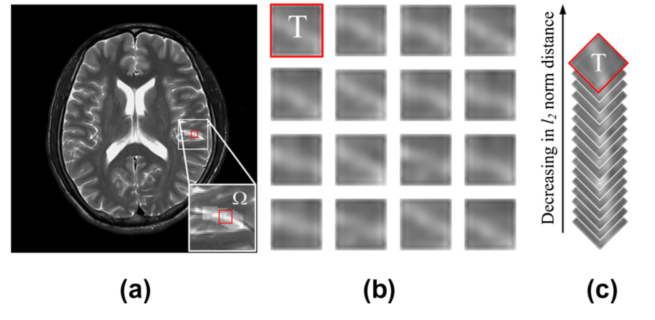
\includegraphics[scale=1]{./image/Group.png}
	\caption{Illustration of the similar patches found via block matching and the sparsity results in. (a) A search region $\Omega$ with $D \times D = 3 9 \times 39$ and the reference patch T with
		$L \times L = 8 \times 8$; (b) Q = 16 similar patches found by the $l_2$ norm distance measure with patch size $L = 8$; (c) 3D array stacked from the similar patches.}
	\label{Group}
\end{figure}
\newpage
\section{Learn the nonlocal similarity from the guide image}
\par The nonlocal similarity is learnt from a fully sampled iamge, and the fully sampled image is reconstrcuted by undersampled data using conventional CS-MRI method. The flowchart of the proposed method  is depicted in Fig \ref{flowchart}.
Firstly, in order to obtain the guide image, a convecntional CS-reconstruction method is performed on undersampled data. Secondly, the block matching is used to acquire nonlocal similarity. Thirdly, the sparsity coefficients of nonlocal similar patches of one group can be produced by PANO. Last, the CS-reconstruction method incorporates PNAO is perfromed to solve the model (\ref{PANOModel}).
\begin{figure}[ht]
	\centering
	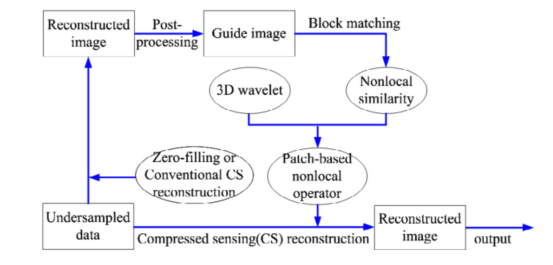
\includegraphics[scale=1]{./image/flowchart.png}
	\caption{ Flowchart  of  the  proposed  PANO-based  MRI  reconstruction  from  undersampled data.}
	\label{flowchart}
\end{figure}
\end{document}